\section{Resumo}
O subsistema de software está presente na interação máquina usuário englobando a gerência de pontuação pelo aplicativo, o reconhecimento do usuário e o reconhecimento e validação da garrafa. A integração será feita diretamente com o subsistema de eletrônica por meio da comunicação de requisições HTTP e indiretamente por meio de leituras de dados dos componentes eletrônicos, como a camêra frontal da máquina e o leitor de garrafa.

Para melhor descrição de alto nível do aplicativo, foi elaborado um documento de visão encontrado nos anexos, onde nele se encontram intervalos de qualidade, requisitos funcionais e diversos tópicos relevantes para sua elaboração.

A equipe de software também é responsável pela estrutura do banco de dados e pelo desenvolvimento da API que fará papel de interface de acesso ao BD, onde tanto o aplicativo quanto a Raspberry PI realizarão requisições.

\section{Prototipação}
Para a otimização do levantamento de Requisitos, foram realizadas reuniões com a equipe de eletrônica para poder nivelar os padrões e protocolos de comunicação entre os dois subsistemas. O protótipo inicial de comunicação ficou da seguinte forma:

\begin{figure}[!ht]
	\centering
		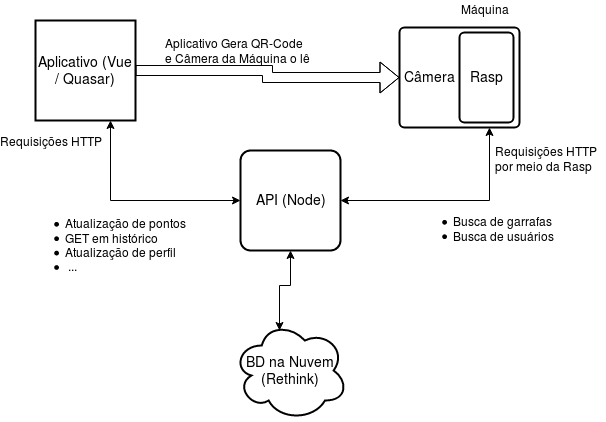
\includegraphics[scale=0.4]{figuras/software/1-prototipo-comunicacao.png}
	\caption{Protótipo de comunicação entre software e hardware.}
\end{figure}

Em relação aos requisitos do aplicativo, foram usados como suporte para levantamento e otimização, o documento de visão(em anexo), o diagrama de caso de uso e protótipos de alto nível (estes estão sendo utilizados nas descrições das funcionalidades no tópico seguinte).

\begin{figure}[!ht]
	\centering
		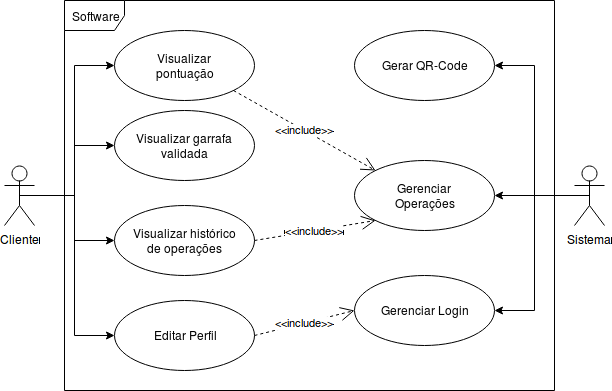
\includegraphics[scale=0.4]{figuras/software/2-Diagrama-de-Caso-de-Uso.png}
	\caption{Diagrama de Caso de Uso.}
\end{figure}

\section{Arquitetura}

A arquitetura do sistema está detalhada no documento de arquitetura em anexo.

\section{API}

Como é descrito no documento de arquitetura em anexo, a API foi desenvolvida utilizando \textit{Node.js} e será acessada por meio de requisições \textit{HTTP}. Além disso, utilizou-se quando possível o estilo de arquitetura \textit{REST} sempre que for possível. Este estilo faz o reúso de URL's endereçáveis, mudando-se apenas o método da requisição. Quando isso não for possível, deve-se aplicar o estilo \textit{RPC}. Este estilo por sua vez não faz o reúso das URL's, mudando a URL e mantendo o método de requisição geralmente como \textit{GET} e \textit{POST}.

A imagem \ref{fig:rest} apresenta um exemplo de implantação de arquitetura \textit{REST}, endereçada previamente sobre a URL \textit{'/user'}.

\begin{figure}[!ht]
	\centering
		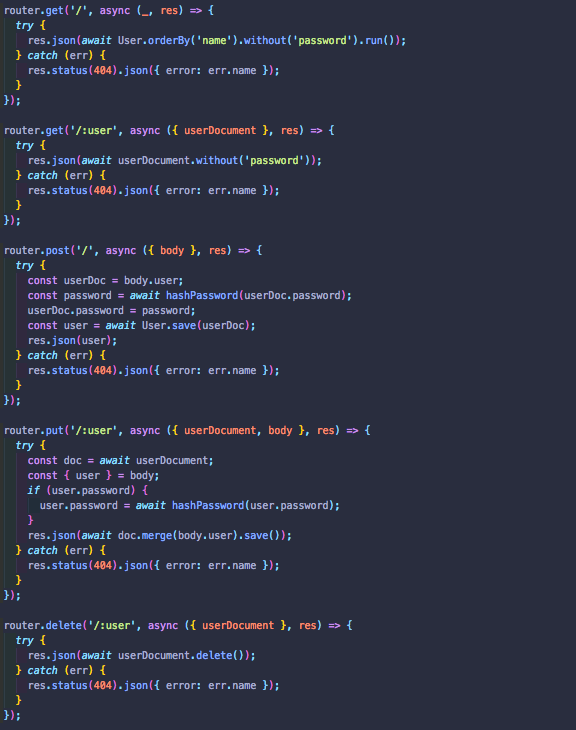
\includegraphics[scale=0.6]{figuras/software/rest.png}
	\caption{Exemplo de implementação de uma arquitetura REST}
	\label{fig:rest}
\end{figure}

Como é possível observar na figura \ref{fig:rest}, o que difere entre as rotas da API são os métodos utilizados na requisição e os parâmetros recebidos dentro da rota, sendo que nenhum altera o endereço estabelecido.

A imagem \ref{fig:rpc} apresenta um exemplo de implantação de arquitetura \textit{RPC}, endereçada previamente sobre a URL \textit{'/user'}.

\begin{figure}[!ht]
	\centering
		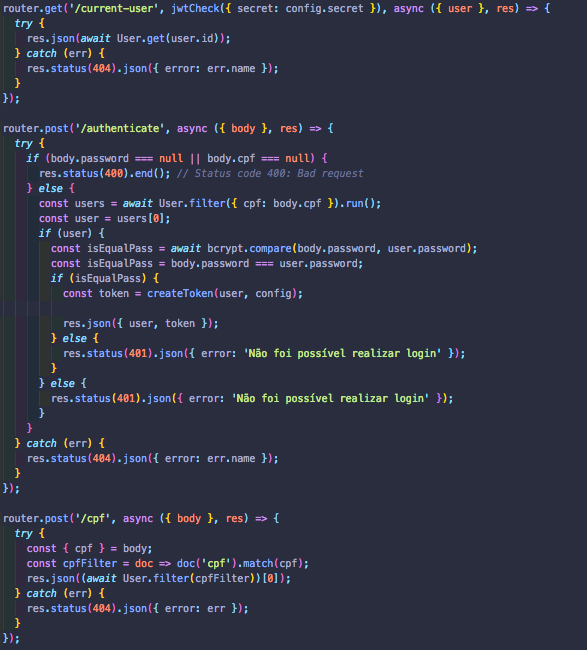
\includegraphics[scale=0.6]{figuras/software/rpc.png}
	\caption{Exemplo de implementação de uma arquitetura RPC}
	\label{fig:rpc}
\end{figure}

Como é possível observar na figura \ref{fig:rpc}, as rotas da API sempre diferem da previamente estabelecida, adicionando-se sempre uma palavra que remete ao propósito daquela rota.

\section{Banco de dados}

Como é descrito no documento de arquitetura em anexo, o banco de dados escolhido é o \textit{RethinkDB}. Tendo em vista que a gerência de banco de dados é feita pela API, sua modelagem fica responsável também pela API. A API por sua vez gerencia o banco de dados através da camada da Model. A imagem \ref{fig:model} representa um exemplo de implementação.

\begin{figure}[!ht]
	\centering
		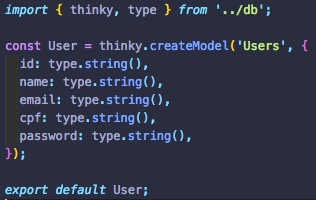
\includegraphics[scale=1]{figuras/software/model.png}
	\caption{Exemplo de implementação de uma Model}
	\label{fig:model}
\end{figure}

Nessa implementação, a comunicação com o banco de dados é feita através de uma aplicação \textit{ORM}, a qual tem a função de realizar todas as \textit{queries} no banco de dados de forma segura através de métodos pré estabelecidos. Dessa forma, como é possível ver na imagem \ref{fig:model}, para criar uma model é utilizado o método \textit{createModel} da \textit{ORM} do \textit{RethinkDB}, o \textit{thinky}.

\section{Integração}

Para que seja feita a integração com a API, devem ser realizadas requisições HTTP sobre as rotas da API. A figura \ref{fig:python} representa um exemplo de implementação de um código em Python o qual comunica com a API e recupera as informações de um usuário com base em seu CPF, que é exatamente o que será feito no projeto.

\begin{figure}[!ht]
	\centering
		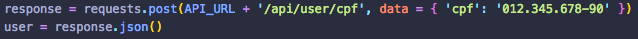
\includegraphics[scale=0.7]{figuras/software/python.png}
	\caption{Exemplo de implementação de uma HTTP request em Python}
	\label{fig:python}
\end{figure}

\section{Funcionalidades}

Este tópico tem a finalidade de descrever as funcionalidades do aplicativo apontadas no diagrama de caso de uso.

\subsection{Login}

Essa funcionalidade envolve primeiro na escolha entre realizar o ato de login quando o usuário já possui uma conta, ou se cadastrar no sistema caso o usuáiro não possua uma conta ainda. No caso de já possuir uma conta, o login deve ser feito fornecendo CPF e Senha. Todas as informações do cadastro são validadas e a senha é criptografada no ato do cadastro.

As imagens em \ref{fig:login} representam o resultado final da implementação dessa funcionalidade.

\begin{figure}[!ht]
	\centering
		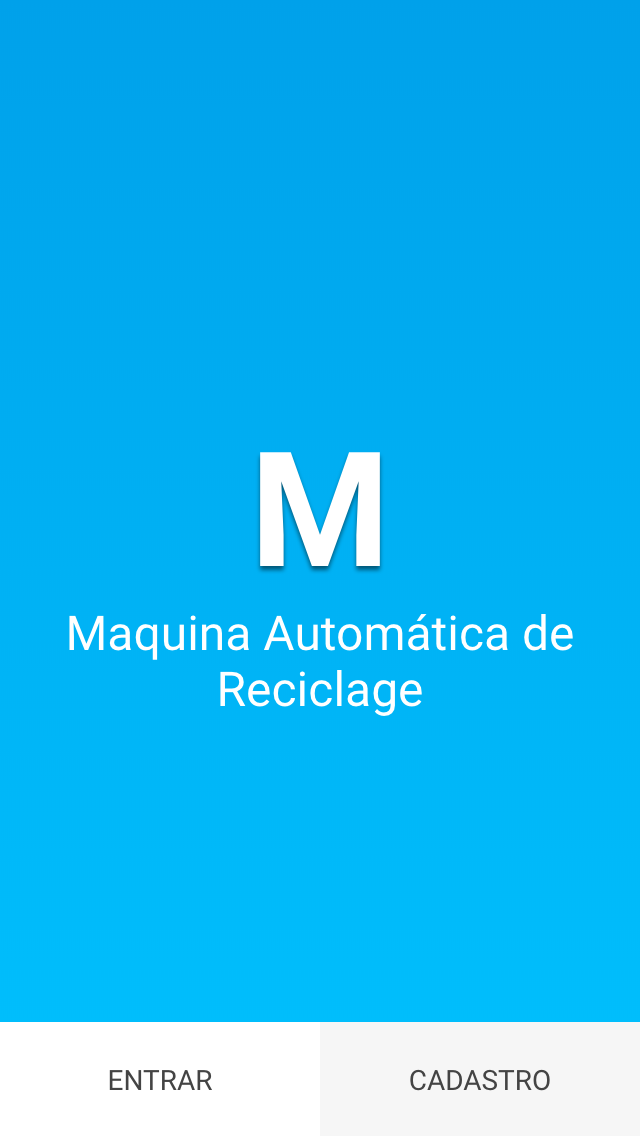
\includegraphics[scale=0.2]{figuras/software/get-in.png}
		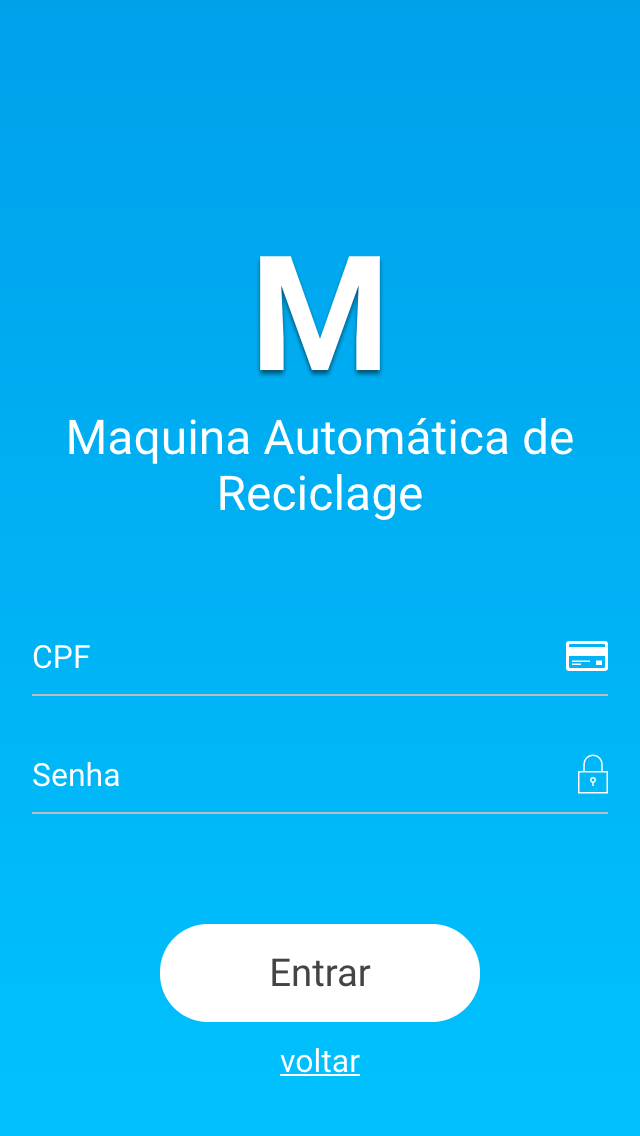
\includegraphics[scale=0.2]{figuras/software/login.png}
		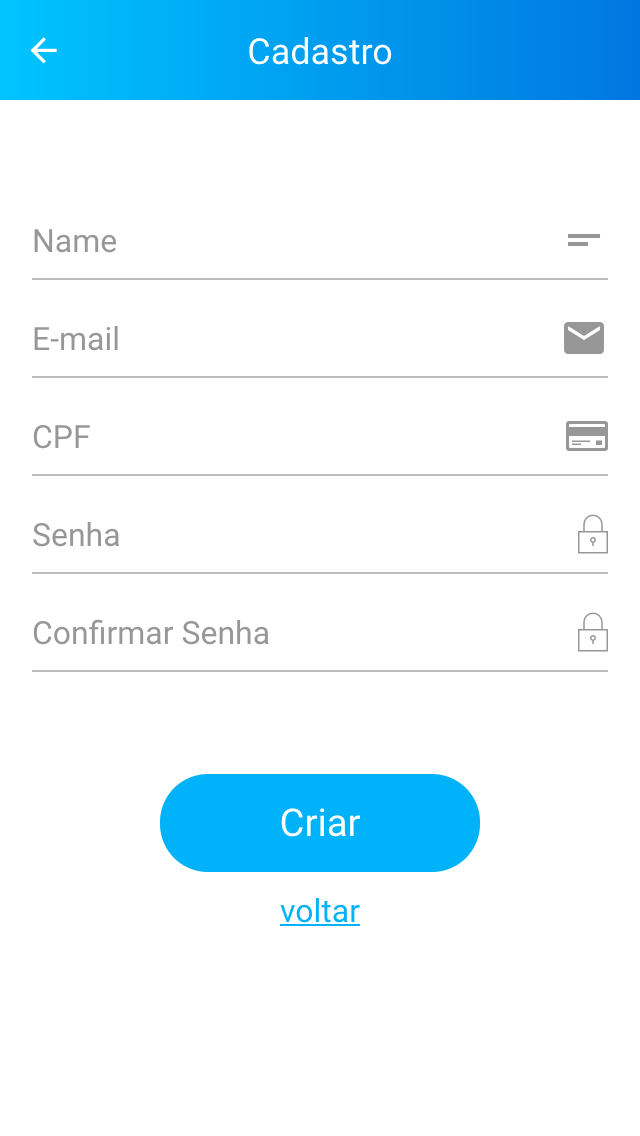
\includegraphics[scale=0.2]{figuras/software/signup.png}
	\caption{Telas de escolha, Login e Cadastro}
	\label{fig:login}
\end{figure}

\subsection{Gerar QR Code}

Essa funcionalidade envolve a geração do QR Code com base no CPF do usuário. Para isso, foi utilizada uma biblioteca que funciona juntamente com o Vue.js. Dessa forma, é gerado um QR Code que quando lido devolve a informação do CPF do usuário. É a primeira tela com a qual o usuário se depara ao entrar na aplicação.

A imagem \ref{fig:qrcode} representa o resultado final da implementação dessa funcionalidade.

\begin{figure}[!ht]
	\centering
		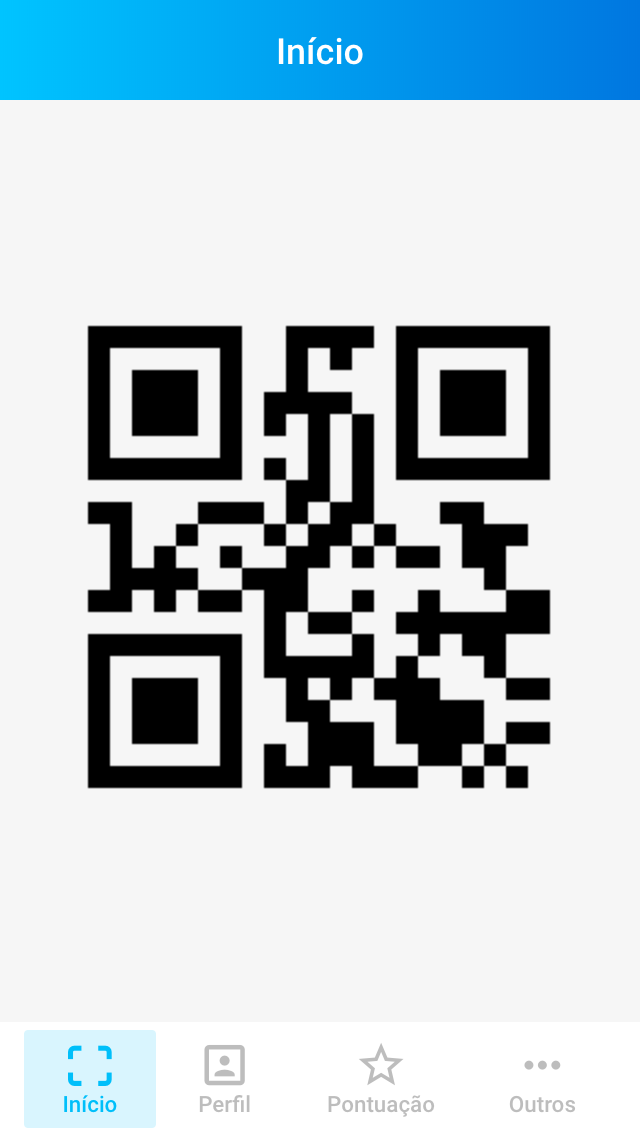
\includegraphics[scale=0.2]{figuras/software/qr_code.png}
	\caption{Tela de início com o QR Code do usuário}
	\label{fig:qrcode}
\end{figure}

\subsection{Visualisar e editar perfil}

Essa funcionalidade envolve o usuário visualizar suas informações cadastradas e poder edita-las. As informações estão dispostas em um componente destacado. O mesmo componente possui um botão para trocar o componente de visualização para um componente de edição. Assim é possível editar as informações, o botão é trocado por um botão de salvar e quando é clicado, o mesmo salva as informações do usuáiro e o componente volta a ser o de visualização.

Foi utilizado o Gravatar para disponibilizar uma imagem de usuário com base em seu e-mail. O Gravatar consiste em um serviço de disponibilização de avatares via associação a e-mails cadastrados. Sua escolha foi feita com base na simplicidade da solução com base no tempo hábil.

A imagem \ref{fig:user} representa o resultado final da implementação dessa funcionalidade.

\begin{figure}[!ht]
	\centering
		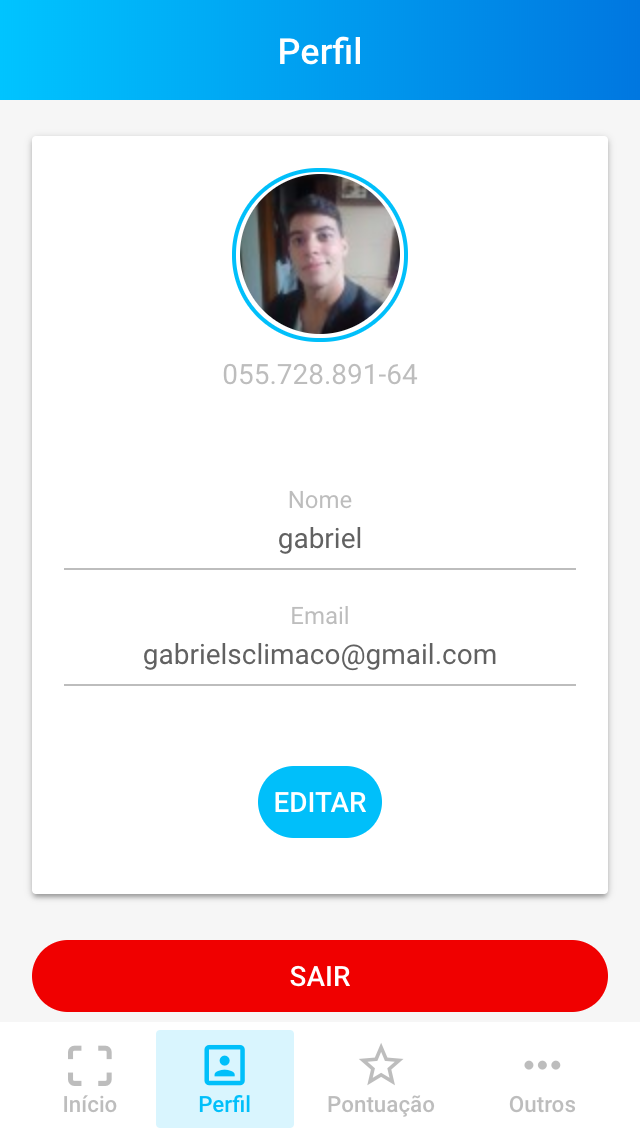
\includegraphics[scale=0.2]{figuras/software/profile.png}
		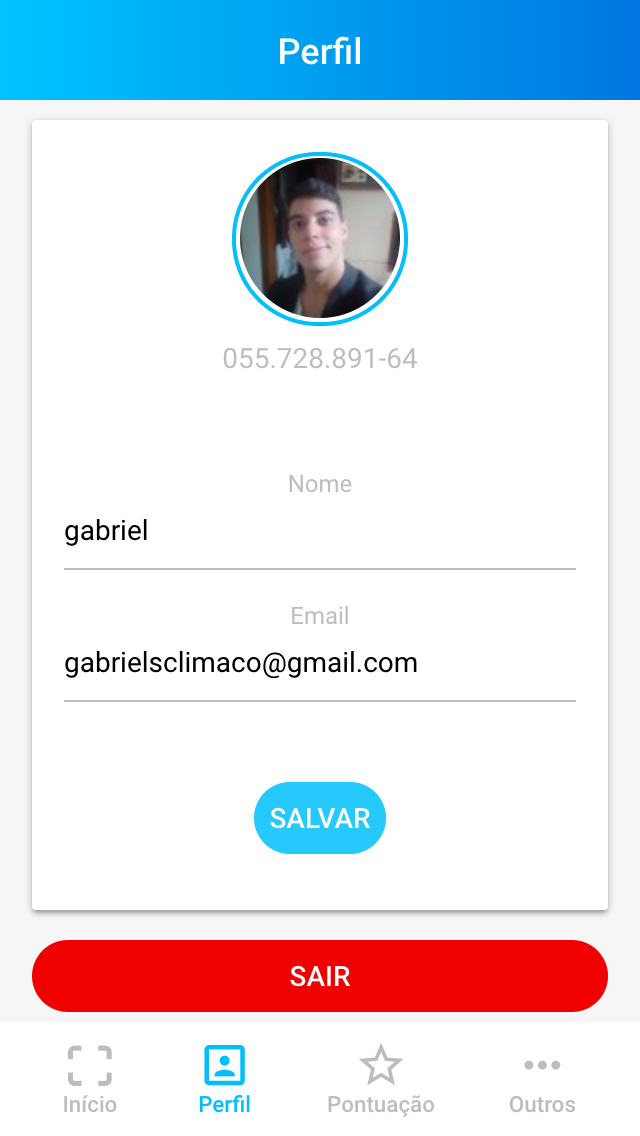
\includegraphics[scale=0.2]{figuras/software/edit.png}
	\caption{Telas de visualização e edição de informações do usuário}
	\label{fig:user}
\end{figure}

\subsection{Visualização do histórico de operações}

Essa funcionalidade envolve visualização das operações de inserção de dados na máquina. As operações estarão dispostas em formato de lista e ordenadas por datas.

A imagem \ref{fig:operation} representa o resultado final da implementação dessa funcionalidade.

\begin{figure}[!ht]
	\centering
		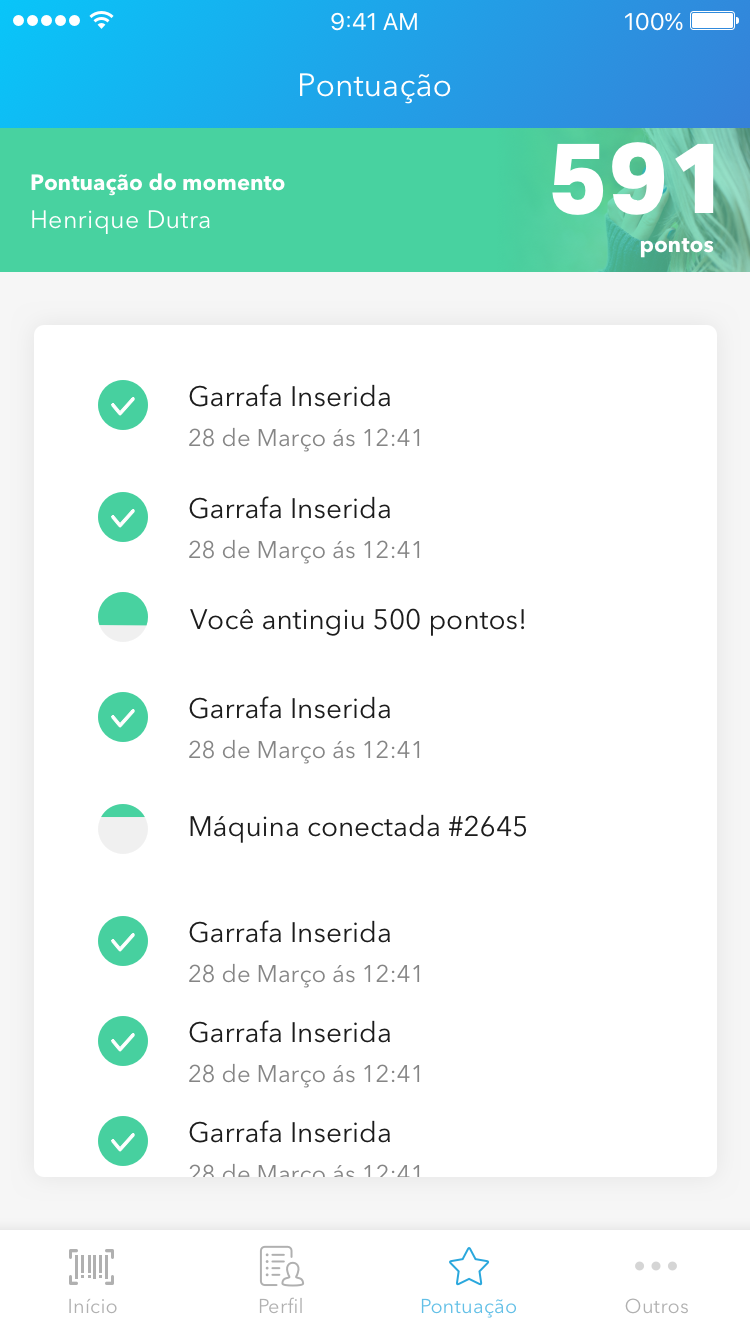
\includegraphics[scale=0.2]{figuras/software/pontuacao.png}
	\caption{Telas de visualização das operações}
	\label{fig:operation}
\end{figure}

\section{Testes}

\subsection{App}

Para testar o aplicativo, foram realizados diversos testes de usabilidade com conhecidos dos integrantes do grupo.

\subsection{API}

Para testar a API, foi utilizado o framework de testes AVA, o qual consiste em uma biblioteca para testes asíncronos em Node.js.
